\section{Continuous-time birth--death and quasi-stationarity}
\label{sec:continuous-bd}

We turn to the linear birth--death process in continuous time. The same subcritical phenomena appear here as in discrete time---certain extinction, together with a non-trivial conditional mean given survival---but now the reciprocal of that conditional mean is elementary in the rates. That contrast with the discrete $A(p)$ is the main structural point of the section. Along the way we record the master-equation bridge to a \pgf\ partial differential equation, so that the method of characteristics later in the chapter is not a cold open.

\subsection{Process and mean ODE}
\label{sec:ct-bd-def}

Let $\xt$ be a continuous-time Markov chain on $\{0,1,2,\ldots\}$ with per capita birth rate $\beta\geq 0$ and death rate $\mu\geq 0$, so that for $n\geq 1$ and small $\delt>0$,
\begin{align*}
\pr{\xx_{t+\delt}=n+1\mid \xt=n}
&=
\beta n\,\delt + o(\delt),
\\
\pr{\xx_{t+\delt}=n-1\mid \xt=n}
&=
\mu n\,\delt + o(\delt),
\end{align*}
with $0$ absorbing. Write $N=\xx_0$ for the initial count, taken deterministic. Because the rates are linear in $n$, the unconditional mean $M(t)=\mean{\xt}$ closes on itself and satisfies
\begin{equation}
\label{eq:mean-ode}
\ddt{M}
=
(\beta-\mu)M,
\qquad
M(0)=N,
\end{equation}
hence $M(t)=N\,\ee^{(\beta-\mu)t}$ whenever the mean exists. The process is subcritical, critical, or supercritical according as $\beta-\mu$ is negative, zero, or positive.

\subsection{Survival probability}
\label{sec:ct-survival}

The extinction probability $p_0(t)=\pr{\xt=0}$ for the linear birth--death process is classical. With initial condition $\xx_0=N$,
\begin{equation}
\label{eq:p0-allen}
p_0(t)
=
\begin{cases}
\displaystyle
\lrb{\frac{\mu - \mu \ee^{(\mu - \beta) t }}{  \beta  - \mu \ee^{(\mu - \beta) t }}}^N,
&
\beta \neq \mu,
\\[1.2em]
\displaystyle
\lrb{\frac{\beta t}{1 + \beta t}}^N,
&
\beta = \mu.
\end{cases}
\end{equation}
(The formula is written here with birth rate $\beta$ in place of the $\lambda$ of many textbooks.) The survival probability is then $S^{(N)}(t)=1-p_0(t)$, and the $N$th power in \eqref{eq:p0-allen} records that the $N$ founding lineages must all die out independently.

\subsection{Limiting conditional mean}
\label{sec:ct-cond-mean}

On the event of non-extinction,
\begin{equation}
\label{eq:condit}
\mean{\xt \mid \xt > 0}
=
\frac{\mean{\xt}}{S^{(N)}(t)}.
\end{equation}
In the \emph{subcritical} regime $\beta<\mu$ both numerator and denominator tend to zero, and L'H\^{o}pital's rule---or, equivalently, direct asymptotics of \eqref{eq:p0-allen}---yields a finite positive limit, which under standard linear rates does not depend on the initial count $N$:
\begin{equation}
\label{eq:ct-qs-mean}
\lim_{t\to\infty}
\mean{\xt \mid \xt > 0}
=
\frac{\mu}{\mu - \beta}
=
\frac{1}{1 - \beta/\mu}.
\end{equation}
The quasi-stationary mean size is thus an explicit rational function of the two rates, and it depends on them only through the ratio $\beta/\mu$.

For a single ancestor ($N=1$) and $\beta\neq\mu$, equations~\eqref{eq:p0-allen}--\eqref{eq:condit} likewise give a closed conditional mean at finite time; its large-$t$ limit is again \eqref{eq:ct-qs-mean} when $\beta<\mu$.

\subsection{Continuous-time analogue of $A(p)$}
\label{sec:continuous-A}

In discrete time the reciprocal of the limiting conditional mean was $A(p)$. The counterpart suggested by \eqref{eq:ct-qs-mean} is therefore the dimensionless factor
\begin{equation}
\label{eq:A-cont}
A_{\mathrm{ct}}(\beta,\mu)
:=
\frac{\mu-\beta}{\mu}
=
1 - \frac{\beta}{\mu},
\qquad
\beta<\mu,
\end{equation}
so that
\[
\lim_{t\to\infty}
\mean{\xt \mid \xt > 0}
=
\frac{1}{A_{\mathrm{ct}}(\beta,\mu)}.
\]
(The notation $A_{\mathrm{ct}}$ is used here for the reciprocal limiting conditional mean in the subcritical regime, independent of $N$ for linear rates.)

A comparison with discrete $A(p)$ requires the two models to be put on one axis, and the natural continuum matching of rates to a division probability is
\begin{equation}
\label{eq:p-from-rates}
p
:=
\frac{\beta}{\beta+\mu}.
\end{equation}
Then $\beta/\mu = p/(1-p)$ and
\begin{equation}
\label{eq:A-cont-p}
A_{\mathrm{ct}}
=
\frac{1-2p}{1-p},
\qquad
p\in\bigl[0,\tfrac12\bigr).
\end{equation}
At $p=0$ one has $A_{\mathrm{ct}}=1$; as $p\to\tfrac12^{-}$, $A_{\mathrm{ct}}\to 0^{+}$ and the conditional mean diverges. Both endpoints are therefore under control for the continuous formula.

Figure~\ref{fig:dtctA} sets $A_{\mathrm{ct}}$, read as a function of $p$ through \eqref{eq:A-cont-p}, against numerical values of the discrete $A(p)$. The two curves have the same shape but not the same normalisation: as noted in Section~\ref{sec:Ap-def}, discrete $A(p)$ lies in $\bigl(0,\tfrac12\bigr]$ and so approaches $\tfrac12$ rather than $1$ as $p\to 0$.

\begin{figure}[ht]
\centering
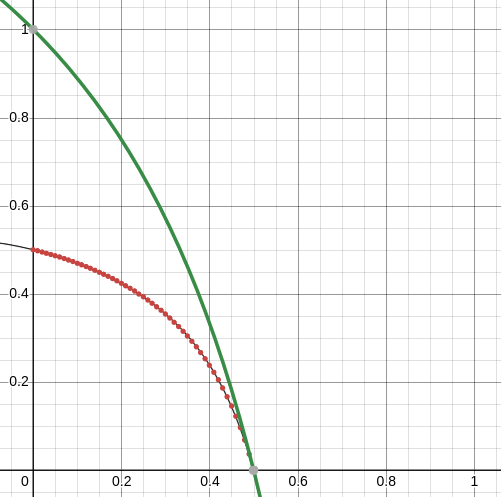
\includegraphics[width=0.55\textwidth]{figures/IMG_ch3/dtctA.png}
\caption{Continuous factor $A_{\mathrm{ct}}=(1-2p)/(1-p)$ (green) against discrete $A(p)$ estimated numerically by iterating \eqref{eq:SnIter} (red). Horizontal axis: effective division probability $p$. (Any additional curve in the source graphic is illustrative only and is not used as a cited closed form.)}
\label{fig:dtctA}
\end{figure}

\paragraph{Core contrast (stated, not proved).}
The continuous subcritical model supplies an elementary closed form for the reciprocal quasi-stationary mean. The discrete factor $A(p)$ is equally well defined as a limit and equally usable in formulae such as \eqref{eq:cond-mean}, yet it is not given by a comparably elementary closed expression on $p\in[0,\tfrac12)$. Path~C returns to that obstruction; Path~A needs only the distinction.

\subsection{Near criticality}
\label{sec:near-critical-philosophy}

As $\beta$ approaches $\mu$ from below, $A_{\mathrm{ct}}\to 0$ and the conditional mean \eqref{eq:ct-qs-mean} becomes arbitrarily large. A process nearly indifferent between gain and loss can therefore, on the rare event of long survival, carry a large typical size without ever having a positive probability of eternal persistence. The same divergence of $1/A(p)$ appears in discrete time as $p\to\tfrac12^{-}$. The point is interpretive rather than a new theorem, but it is the one worth carrying forward: criticality organises not only extinction probabilities but the scale of what survival looks like when it occurs.

\subsection{From the master equation to a \pgf\ PDE}
\label{sec:pgf-bridge}

Let $p_n(t)=\pr{\xt=n}$ and $G(z,t)=\sum_{n\geq 0} p_n(t) z^n=\mean{z^{\xt}}$. Substituting the master equation of Section~\ref{sec:master-eq}, with rates $\beta,\mu$, and rearranging yields the first-order equation
\begin{equation}
\label{eq:pgf-pde-bd}
\pdx{G}{t}
=
\bigl(\beta z^2 - (\beta+\mu)z + \mu\bigr)
\pdx{G}{z},
\end{equation}
for $z\in[0,1]$, with initial condition $G(z,0)=z^{N}$ when $\xx_0=N$.

Equation~\eqref{eq:pgf-pde-bd} is a linear transport equation in $(z,t)$, and it is solved by following the curves along which $G$ does not change. Writing $a(z)=\beta z^2-(\beta+\mu)z+\mu$, so that the PDE reads $G_t=a(z)G_z$, we have along any curve $z(t)$
\[
\frac{\dd}{\dd t}G\bigl(z(t),t\bigr)
=
\bigl(a(z)+\dot z\bigr)G_z.
\]
Hence $G$ is constant on characteristics precisely when
\begin{equation}
\label{eq:char-z}
\dda{z}{t}
=
-a(z)
=
-\bigl(\beta z^2 - (\beta+\mu)z + \mu\bigr)
=
(\beta z-\mu)(1-z).
\end{equation}
(The pure-death case $\beta=0$ gives $\dot z=\mu(z-1)$, matching the explicit solution $G(z,t)=\bigl(1-\ee^{-\mu t}+z\ee^{-\mu t}\bigr)^N$.)

Solving \eqref{eq:char-z} with $G(z,0)=z^N$ recovers the classical closed-form generating function of the linear birth--death process, standard in the textbooks; the single-ancestor case determines the general $N$ case by independence of lineages. In particular $p_0(t)=G(0,t)$ reproduces \eqref{eq:p0-allen}, the formula already used above for survival and conditional means. That closes the loop, and it is the verification the bridge requires: the PDE, the characteristic field \eqref{eq:char-z}, and consistency with the extinction formula.

\paragraph{Exit contract for the method of characteristics.}
The later method-of-characteristics development may therefore assume three things: (i) that a univariate CTMC \pgf\ satisfies a first-order PDE obtained from the master equation; (ii) that for linear birth--death this PDE is \eqref{eq:pgf-pde-bd}, the characteristics are \eqref{eq:char-z}, and the solution is the classical closed form with $p_0=G(0,\cdot)$ as in \eqref{eq:p0-allen}; and (iii) that the same idea extends when the state is multivariate or when further transitions modify the transport field. The method-of-characteristics section develops the absorption ladder (with and without birth and death) in detail; catastrophe rates in full BDC models are taken up in later chapters, reusing the same generating-function pattern.
